% 添加快捷键
fn+F1 搜索 keybingdings.json

% 序号段落样例
\begin{enumerate}
    \item    
\end{enumerate}

% 表格样例
\begin{table}[htbp]
    \centering
    \caption{题目 \label{tab:parameters}}
    \bgroup\def\arraystretch{1.5}
    \setlength{\tabcolsep}{4.5mm}
      \begin{threeparttable}%要写注释,得加这行
        \begin{tabular}{c|c}
          \toprule
          \textbf{11} & \textbf{22}\\
          \midrule\midrule
          \grayrow  & \\
           & \\
          \grayrow  & \\ 
          \bottomrule
        \end{tabular}

        %注释
        \begin{tablenotes}%注释开始
        \footnotesize
        \item[$\ast$] $\mathtt{rand}\ [a, b]\ (a<b)$ is a random value generated between $a$ and $b$.
        \end{tablenotes}%注释结束
      \end{threeparttable}%要写注释,得加这行

    \egroup
\end{table}

% 插入图片样例
\begin{figure}[htbp]
    \centering
    \includegraphics[width=0.7\textwidth]{fig/}
    \caption{}
    \label{fig:}
\end{figure}

% 插入tikz图片
\begin{figure}[hbpt]
    \centering
    \begin{tikzpicture}[node distance = 2cm]
    \definecolor{myblued}{RGB}{0,114,189}
    \definecolor{myred}{RGB}{217,83,25}
    \definecolor{myyellow}{RGB}{237,137,32}
    \definecolor{mypurple}{RGB}{126,47,142}
    \definecolor{myblues}{RGB}{77,190,238}
    \definecolor{mygreen}{RGB}{32,134,48}
      \pgfplotsset{
        label style = {font=\fontsize{9pt}{7.2}\selectfont},
        tick label style = {font=\fontsize{7pt}{7.2}\selectfont}
      }
    
    \small  % 字体大小
    \tikzstyle{format}=[rectangle,draw,thin,fill=white]  % 定义语句块的颜色,形状和边
    % rectangle:矩形,可加圆角(rounded corners,逗号跟在形状后面即可)
    % trapezium:平行四边形
    % diamond:菱形
    \tikzstyle{test}=[diamond,aspect=2,draw,thin]  % 定义条件块的形状,颜色
    \tikzstyle{point}=[coordinate,on grid,]  % 像素点,用于连接转移线

    % 定义note
    \node[format](asm){在记事本事先编好程序,并修改后缀名为\texttt{.asm}};
    \node[format,below of=asm,node distance=10mm](masm){使用命令\texttt{masm yourfile.asm}生成目标文件};
    \node[test,below of=masm,node distance=20mm](if){0 wornings, 0 errors?};
    \node[format,below of=if,node distance=20mm](link){使用命令\texttt{link yourfile}进行连接操作};
    \node[format,below of=link,node distance=10mm](execute){执行\texttt{youfile.exe}文件};
    % 开始画线
    \draw[->](asm)--(masm);
    \draw[->](masm)--(if);
    \draw[->](if)--node[left]{Yes}(link);
    \draw[->](link)--(execute);
    \draw[->](if.west) -+ (-5,-3) -+ node[left]{No}(-5,0) -- (asm.west);
    % \draw[-](point2) to [in=-90,out=90];
    % \draw[->](point2)--(asm.west);
\end{tikzpicture}
    
    \caption{图片}
    \label{fig:xxx}
\end{figure}

% 并排两张图样例
\begin{figure}[htbp]
    \centering
    \subfloat[原理图]{
        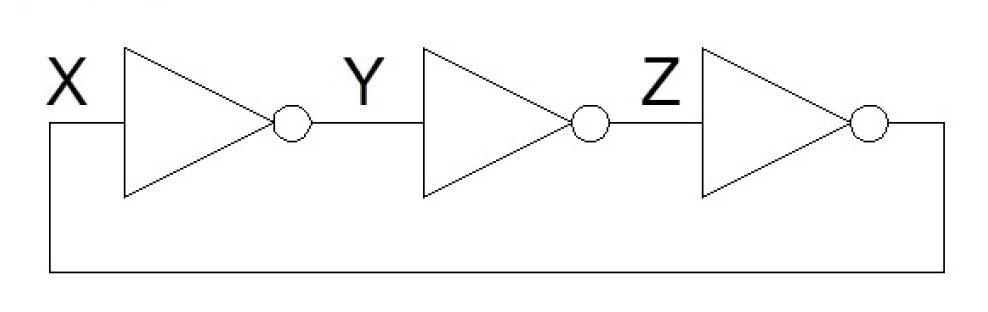
\includegraphics[height=2cm]{fig/oscillation_init.png}
        \label{subfig:oscillation_init}
    }
    \subfloat[等效图]{
        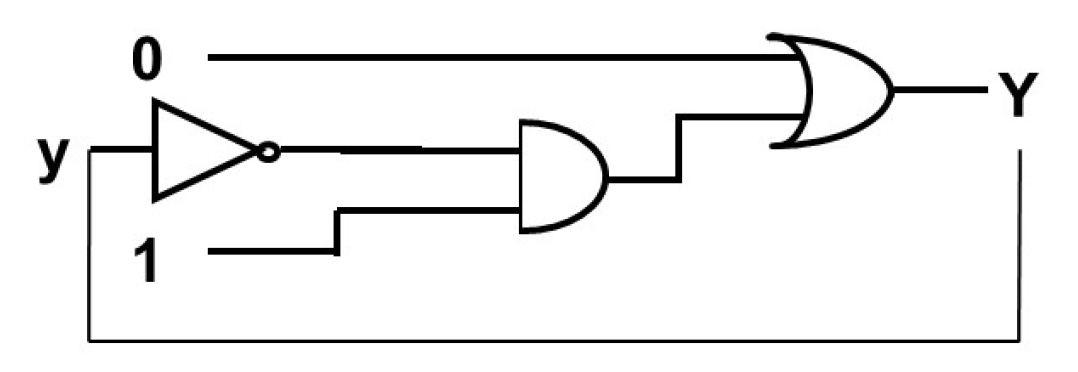
\includegraphics[height=2cm]{fig/oscillation_real.png}
        \label{subfig:oscillation_real}
    }
    \caption{}
    \label{fig:oscillation_circuit}
\end{figure}

% 注意样例(idea/analyze 分别表示思考和分析)
\begin{note}{题目}{}
    内容
\end{note}

% 代码样例
\begin{lstlisting}[language={[x86masm]Assembler},title=code]
    
\end{lstlisting}